\documentclass[fleqn,10pt]{wlscirep}
\usepackage[utf8]{inputenc}
\usepackage[T1]{fontenc}
\title{Direction-selective Resistance to Cerebrospinal Fluid Flow as The
Mechanism of Syrinx Generation in Syringomyelia}

\author{Han Soo Chang, M.D.}
\affil{Department of Neurosurgery, Tokai University\\Isehara, Japan}

\keywords{syringomyelia, pathophysiology, simulation}

\begin{abstract}
Example Abstract. Abstract must not include subheadings or citations. Example Abstract. Abstract must not include subheadings or citations. Example Abstract. Abstract must not include subheadings or citations. Example Abstract. Abstract must not include subheadings or citations. Example Abstract. Abstract must not include subheadings or citations. Example Abstract. Abstract must not include subheadings or citations. Example Abstract. Abstract must not include subheadings or citations. Example Abstract. Abstract must not include subheadings or citations.
\end{abstract}
\begin{document}

\flushbottom
\maketitle
% * <john.hammersley@gmail.com> 2015-02-09T12:07:31.197Z:
%
%  Click the title above to edit the author information and abstract
%
\thispagestyle{empty}

\noindent Please note: Abbreviations should be introduced at the first mention in the main text – no abbreviations lists. Suggested structure of main text (not enforced) is provided below.

\section*{Introduction}

The pathophysiology of syringomyelia is still poorly understood. A number
of hypotheses exist in the literature [@gardner1958mechanism;
@williams1980pathogenesis; @milhorat1999chiari; @ball1972pathogenesis;
@klekamp2002pathophysiology; @duboulay1974mechanism; @heiss1999elucidating;
@milhorat1993anatomical; @stoodley2000pathophysiology; @terae1994increased;
@chang2003hypothesis; @chang2004theoretical; @greitz2006unraveling], but
they provide widely different explanations on the mechanisms of syrinx
generation.  Most researchers, nevertheless, seem to agree on the following
points. First, the syrinx fluid is identical to the CSF, and there should
be some communication between the syrinx and the subarachnoid space. This
point is supported by many studies [@ellertsson1969syringomyelia;
@ellertsson1969myelocystographic; @li1987conventional; @heiss2019origin],
although a few different opinions exist [@greitz2006unraveling;
@koyanagi1997surgical]. Second, some derangement of CSF flow in the spinal
subarachnoid space causes syrinx both in Chiari-I malformation
[@wolpert1994chiari; @bhadelia1995cerebrospinal; @heiss1999elucidating;
@hofmann2000phasecontrast; @quigley2004cerebrospinal] and subarachnoid
arachnopathy [@klekamp1997treatment; @brodbelt2003altered;
@heiss2012pathophysiology; @chang2014dorsal]. The cerebellar tonsils hamper
the CSF flow in the former and adhesive arachnoiditis in the latter.

The problem, however, is where this communicating channel resides and what
mechanism generates the syrinx. On these points, there is no solid
experimental or clinical evidence, and the opinions of researchers deviate
widely. Gardner et al. [@gardner1958mechanism] thought that the central
canal intercommunicates the syrinx and the fourth ventricle, and arterial
pressure waves exerted on the central canal generate the syrinx. Williams
et al. also postulated the communication through the central canal, but for
the syrinx generation mechanism, he emphasized the craniospinal pressure
gradient produced by Valsalva maneuver et al.  On the other hand, Ball and
Dayan [@ball1972pathogenesis] assumed that CSF enters the syrinx through
the perivascular space of arteries penetrating the spinal cord. This idea
has the following variations. Heiss et al. [@heiss1999elucidating] proposed
that the piston-like movement of the cerebellar tonsils in Chiari-I
patients generates pressure waves in the spinal subarachnoid space, which
subsequently drive CSF into the syrinx through the perivascular space.
Stoodley et al. also considered the perivascular space as the communicating
channel, but he assumed the arterial pulse pressure as the driving force of
CSF [@stoodley2000mechanisms]

All these assumptions are not proven and remain hypothetical. Although the
perivascular-space theory seems to be favored by recent researchers, there
remains the possibility that a thin communicating channel exists between
the syrinx and the fourth ventricle [@chang2021hypothesis].  In our
opinion, the main theoretical problems reside in the following points.
\begin{enumerate}
    \item No theory can explain the pathophysiological mechanism of syringomyelia in a unified fashion.
    \item No theory can explain how CSF enters from the low-pressure subarachnoid space to the high-pressure syrinx cavity and remains inside.
\end{enumerate}

As to the first point, there are different syringomyelia types, such as
Chiari-I-malformation and spinal-arachnopathy-related. The
Chiari-I-malformation-related syringomyelia is further divided into
communicating and non-communicating. For each of them, current theories
assume a distinct mechanism of syrinx generation. However, it may be more
natural to conjecture some common mechanism underlying these different
types of syringomyelia [@stoodley2000mechanisms].  The second point is
theoretically essential but challenging to solve. Physical theories dictate
that the expanded syrinx cavity has higher pressure than the subarachnoid
space [@serwayr.a.2016fluids; @heiss1999elucidating; @davis1989mechanisms;
@ellertsson1970distending]. Therefore, merely assuming a communicating
channel does not explain how CSF enters the syrinx and remains inside
against this pressure gradient. Even if we take a specific time window
where the subarachnoid pressure exceeds the syrinx pressure, it does not
explain how the CSF remains inside the syrinx after it.

The current article is part of our effort to solve the above theoretical
problems. In our previous paper [@chang2021hypothesis], we hypothesized
that if there is a resistance to CSF flow in a particular direction
(rostral or caudal), it causes a one-way valve-like effect on a CSF channel
inside the spinal cord, leading to the accumulation of CSF and generation
of a syrinx. This hypothesis could explain the pathophysiology of both
Chiari-I-malformation-related syringomyelia and arachnopathy-related
syringomyelia. In Chiari-I-malformation-related syringomyelia, the
herniated cerebellar tonsils may function as a direction-selective
resistance. In arachnopathy-related syringomyelia, some arachnoid adhesion
may play the same function.  However, in that article, we just drew a rough
sketch of this process and left out a detailed explanation. The current
article will describe in detail how direction-selective resistance in the
subarachnoid space generates a one-way valve mechanism in the CSF channel
inside the spinal cord.

For this purpose, we used a mathematical model simulating the CSF movement
of the spine—a revised version of our previous model [@chang2003hypothesis;
@chang2004theoretical]. This model describes the spinal CSF movement as an
electric current in a modeled circuit (a lumped parameter model with
multiple compartments [@shi2011review]), and it assumes the existence of a
patent central canal. We placed a direction-selective resistance in this
model at a certain point in the spinal subarachnoid space and observed how
it affects the CSF flow in the central canal.  \section*{Results}


\section*{Discussion}

The Discussion should be succinct and must not contain subheadings.

\section*{Methods}

Topical subheadings are allowed. Authors must ensure that their Methods section includes adequate experimental and characterization data necessary for others in the field to reproduce their work.

\bibliography{sample}

\noindent LaTeX formats citations and references automatically using the bibliography records in your .bib file, which you can edit via the project menu. Use the cite command for an inline citation, e.g.  \cite{Hao:gidmaps:2014}.

For data citations of datasets uploaded to e.g. \emph{figshare}, please use the \verb|howpublished| option in the bib entry to specify the platform and the link, as in the \verb|Hao:gidmaps:2014| example in the sample bibliography file.

\section*{Acknowledgements (not compulsory)}

Acknowledgements should be brief, and should not include thanks to anonymous referees and editors, or effusive comments. Grant or contribution numbers may be acknowledged.

\section*{Author contributions statement}

Must include all authors, identified by initials, for example:
A.A. conceived the experiment(s),  A.A. and B.A. conducted the experiment(s), C.A. and D.A. analysed the results.  All authors reviewed the manuscript. 

\section*{Additional information}

To include, in this order: \textbf{Accession codes} (where applicable); \textbf{Competing interests} (mandatory statement). 

The corresponding author is responsible for submitting a \href{http://www.nature.com/srep/policies/index.html#competing}{competing interests statement} on behalf of all authors of the paper. This statement must be included in the submitted article file.

\begin{figure}[ht]
\centering
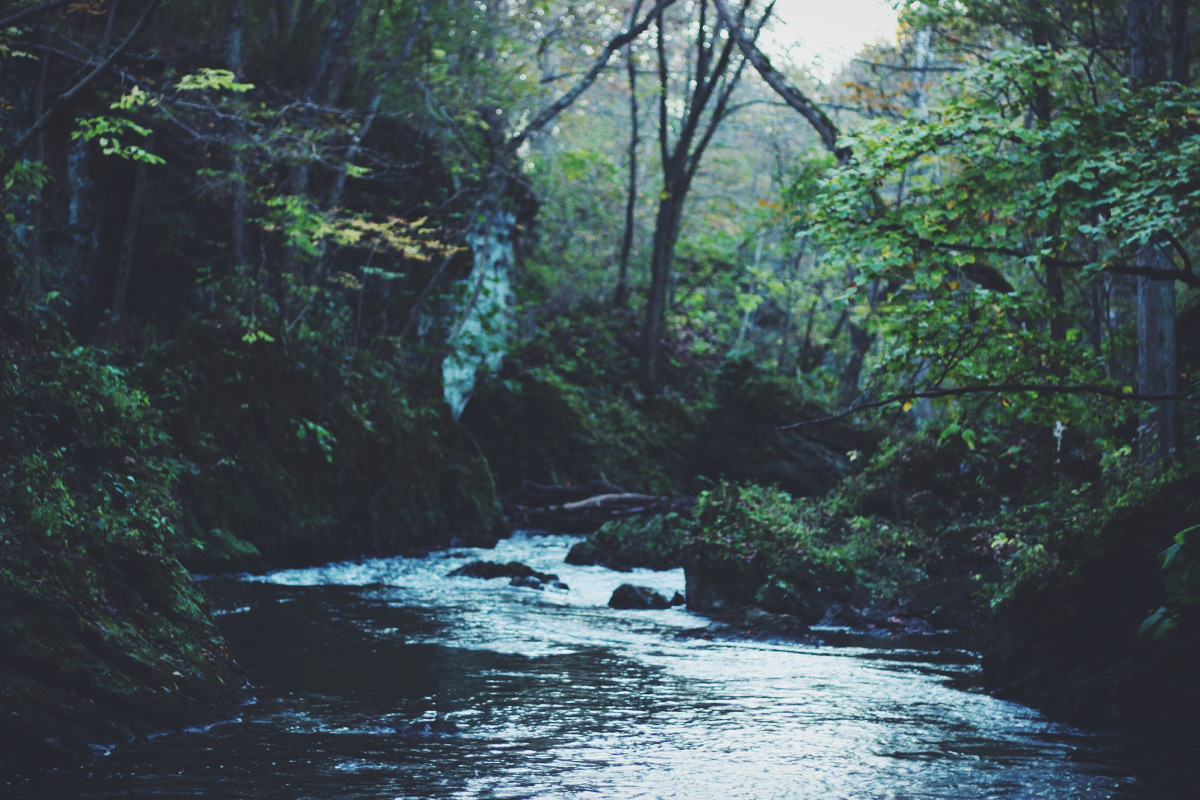
\includegraphics[width=\linewidth]{stream}
\caption{Legend (350 words max). Example legend text.}
\label{fig:stream}
\end{figure}

\begin{table}[ht]
\centering
\begin{tabular}{|l|l|l|}
\hline
Condition & n & p \\
\hline
A & 5 & 0.1 \\
\hline
B & 10 & 0.01 \\
\hline
\end{tabular}
\caption{\label{tab:example}Legend (350 words max). Example legend text.}
\end{table}

Figures and tables can be referenced in LaTeX using the ref command, e.g. Figure \ref{fig:stream} and Table \ref{tab:example}.

\end{document}
